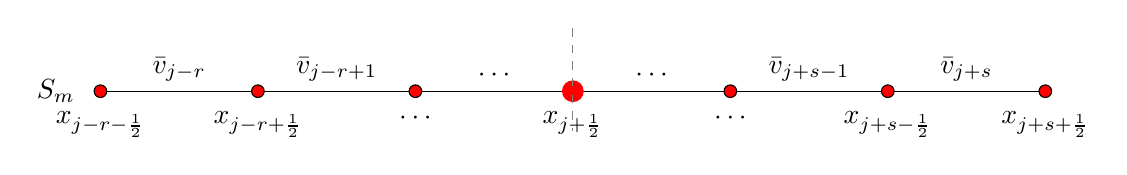
\begin{tikzpicture}[>=stealth]

    % 参数：r=2, s=1 为示例（共 n+1=4 个节点，对应 n=3）
    % 节点位置：x_{j-r-1/2} 到 x_{j+s+1/2}
    % 对应界面：j-5/2, j-3/2, j-1/2, j+1/2, j+3/2
    % 对应单元均值：j-2, j-1, j, j+1

    % ---------- 单元均值标注（上方）----------
    \node[above] at (1,  0) {$\bar{v}_{j-r}$};
    \node[above] at (3,  0) {$\bar{v}_{j-r+1}$};
    \node[above] at (5,  0) {$\cdots$};
    \node[above] at (7,  0) {$\cdots$};
    \node[above] at (9,  0) {$\bar{v}_{j+s-1}$};
    \node[above] at (11,  0) {$\bar{v}_{j+s}$};

    % ---------- 主数轴 ----------
    \draw (0,0) -- (12,0);

    % ---------- 全局模板 S_m 的界面节点（红色）----------
    \foreach \x/\lbl in {
        0/{$x_{j-r-\frac{1}{2}}$},
        2/{$x_{j-r+\frac{1}{2}}$},
        4/{},
        6/{$x_{j+\frac{1}{2}}$},
        8/{},
        10/{$x_{j+s-\frac{1}{2}}$},
        12/{$x_{j+s+\frac{1}{2}}$}
    }{
        \draw[fill=red] (\x,0) circle (0.08) node[below=4pt] {\lbl};
    }

    % 省略号位置补充标注
    \node[below=4pt] at (4,0) {$\cdots$};
    \node[below=4pt] at (8,0) {$\cdots$};

    % 目标界面 x_{j+1/2} 加粗标记
    \draw[fill=red, draw=red, line width=1pt] (6,0) circle (0.12);

    % S_m 标签
    \node[left] at (-0.2, 0) {$S_m$};

    % ---------- 目标界面竖线 ----------
    \draw[dashed, gray] (6, 0.8) -- (6, -0.5);
    % \node[above, gray] at (6, 0.8) {\footnotesize 目标界面};

    % % ---------- 模板范围括号（下方）----------
    % \draw[decorate, decoration={brace, amplitude=6pt, mirror}]
    %     (0, -0.9) -- (10, -0.9)
    %     node[midway, below=8pt] {$n+1$ 个插值节点};

    % % ---------- 左侧 r 段标注 ----------
    % \draw[<->, blue] (0, -1.6) -- (6, -1.6)
    %     node[midway, below=3pt, blue] {$r+1$ 个节点（左侧）};

    % % ---------- 右侧 s 段标注 ----------
    % \draw[<->, teal] (6, -1.6) -- (10, -1.6)
    %     node[midway, below=3pt, teal] {$s$ 个节点（右侧）};

\end{tikzpicture}
